%!TEX root = main.tex
Most of us probably know the feeling of standing in front of a shelf in the supermarket at the end of a stressful day at work not knowing what to buy, or better, not being able to decide what to buy. Even the tiniest, most unimportant decision seems too difficult to make.\par
In 1998, Roy F. Baumeister, Ellen Bratslavsky, Mark Muraven and Dianne M. Tice gave this phenomenon, which they called ‘ego depletion’, a theoretical foundation. Raising the question “\emph{Is the Active Self a Limited Resource?}” \citep{baumeister1998ego}, they formulated their theory on the assumption of willpower or volition as a scarce resource. Therefore, if one taps into this ‘pool of willpower-energy’ the source diminishes over time. More than that, re-search indicates that the energy, which was formerly used on self-control, has an impact on subsequent decision-making \citep{muraven1998self}. It appears as if self-regulation and acts of choice are drawn from the same source, a theory endorsed by Vohs and Heatherton \citep{vohs2000self}. Findings show that chronic inhibition\footnote{Chronic inhibition leads with situational conditions to the drain of self-regulation energy.\citep{vohs2000self} } requires self-regulation. This chapter will closely examine ego depletion theory, focussing especially on choice and risk, in order to establish a theoretical foundation for ‘social risk’ within the theory’s framework.
\section{Ego Depletion - Willpower as a Scarce Resource}
Ego depletion is a relatively young field of research developed in the early 1990s. Although social scientists and psychologists had addressed the analysis of the inner self and the exhaustion of the mind\footnote{“\emph{The notion that volition depends on the self’s expenditure of some limited resource was anticipated by Freud}“ \citep{baumeister1998ego}} earlier (compare \citep{ross1975perceived} and \citep{brody1968personality}), Roy F. Baumeister \citep{baumeister1998ego} gave the discussion on that topic a new drive. Baumeister, along with Bratslavsky, Muraven and Tice formulated the theory of willpower as a scarce resource and defined the term of ego depletion. „\emph{The core idea behind ego depletion is that the self's acts of volition draw on some limited resource, akin to strength or energy and that, therefore, one act of volition will have a detrimental impact on subsequent volition}“ \citep{baumeister1998ego}. They conducted four experiments. Experiments 1, 2 and 3 aimed at supporting the hypothesis of ego depletion itself with differing approaches, whereas experiment 4 was designed to analyse the effects of ego depletion on subsequent decision-making\footnote{The passive option effect was only noticed under ego depletion. The passive option effect describes a circum-stance in which “\emph{[\ldots] the given option is chosen more when it requires an active respose.}“ \citep{baumeister1998ego}}. Therefore, they came to the assumption that ego depletion as a result of self-regulation leads to weaker performance and passivity in decision-making for at least a short period of time. With different depletion approaches in several experiments they came to the conclusion that “\emph{[\ldots] efforts to control thoughts, feelings, physical endurance, and task persistence all draw from the same limited resource} \citep{muraven1998self}.\par
Two years later Muraven and Baumeister \citep{muraven2000self} published a theoretical paper on that subject in which they reduced this self-control strength model (i.e. ego depletion) to five axioms.
\begin{enumerate} [1.]
\item “\emph{[\ldots] self-control strength is necessary for the executive component of the self [\ldots]}” \citep[p.~248]{muraven2000self}
\item “\emph{[\ldots] self-control strength is limited, in the sense that a person has finite capacity for self-control [\ldots]}” \citep[p.~248]{muraven2000self}
\item “\emph{[\ldots] all self-control operations draw on the same resource. Directing one's self-control ef-forts toward one goal should diminish the resources available for self-control in any other sphere}” \citep[p.~248]{muraven2000self}
\item “\emph{[\ldots] the success or failure of self-control depends on the person's level of self-control strength [\ldots]}” \citep[p.~248]{muraven2000self}
\item “\emph{[\ldots] self-control strength is expended in the process of self-control.}” \citep[p.~248]{muraven2000self}
\end{enumerate}
The results of the data they collected provided the foundation to formulate the suggestion that the act of self-control or self-regulation drains from the general source of willpower, which has an impact on subsequent self-control operations, such as decision-making processes. Furthermore, Muraven et al. postulate that self-control can be trained, leading to an increase of the source. This statement raises the question on the measurement of ego depletion. If will power can be increased over time, is a measure of a depletion group in itself comparable? In other words, someone who is ‘trained’ regarding self-regulation might bias the results in a depletion task.\par
Nevertheless, resource models on self-regulation found support in the empirical and the theoretical research on ego depletion \citep{mischel1996good,gross1998emerging,vohs2000self} .\par
In 2002, Baumeister \citep{baumeister2002yielding}  specified the terms of research by examining the circumstances of choice. For that reason, he distinguished between decisions based on careful deliberation and choices of intuitive thinking. Experiments (for a detailed review see \cite{vohs2000self}) have shown that the consequences resulting from a depleted mind are not limited to mere self-regulation but to choice in general. These findings, backing up Baumeister’s former theory, formulated in 1998, led to the conclusion that depleted states caused by self-regulation often lead to a more intuitive decision-making process \citep{pocheptsova2009deciding}. This concept will be more closely discussed in chapter \ref{chap2.2} \todo{remove}2.2. Moreover, Baumeister’s work involved possible implications for consumer research and the patterns of decision-making, setting new impulses. He defined three axioms for self-control failure: Conflicting goals undermines control, monitoring own behaviour and ego depletion. \par
He concentrated on the strength model\footnote{Baumeister stated that the strength model has proven itself, over the cognitive theory and the theory based in skill, as the most significant to former research \citep{baumeister2012self}} as groundwork for future research. If self-control represents the capacity to resist temptation, then ego depletion might lead to impulsive pur-chases \citep{baumeister2002yielding,baumeister2012self}. “\emph{The strength model can illuminate how self-control operates and functions.}” \cite{baumeister2007strength}\par
Although former research has shown that ego depletion leads to risk-aversion in decision-making, the field of unanswered questions remains wide. Leaving the path of classic ‘measurable’ risk (e.g. financial loss) towards a form of risk which is more difficult to measure or to find a clear definition for, brings us to the first core aspect of this study. \par
While research on ego depletion and the effects on risk behaviour and therefore decision-making has received ample empirical and theoretical attention \citep{vohs2008making,vohs2007spent,unger2011ego}, the field of research on ego depletion and the effects on decision-making under the examination of social risk is still widely neglected. The subtle difference, however, might result in a strong impact on decision-making.\par

\section{Ego Depletion and the Risk of Choice}
Consumption always involves choice. However, with every single choice, we make a decision in favour of something and against something else. The possibility to make the ‘wrong’ decision is always present. Consequently, the risk of choice is more than the decision between two alternatives and demands a closer examination.\par
In 2002 Baumeister \citep{baumeister2002yielding} abandoned the mere discussion of existence of ego depletion towards the question of potential implications regarding decision-making pro-cesses and consequences for consumer choice. Before deepening the concept of risk, however, the term self-control needs to be defined. Self-control or self-regulation, in this context used as synonyms, compares to a TOTE model (test-operate-test-exit), in which behaviour is constantly reviewed, using personal standards, until a desired state is reached. In this case, standards are understood as people’s ambition to control their behaviour. Behaviour underlies a constant screening process with regard to inconsistent tendencies or what can be called one’s personal code of conduct, which ultimately provides the capability to change one’s own behaviour.\par
These three ‘pillars’ (standards, monitoring, and change) can be described as an inter-dependent and constantly repeating process to resist temptation. Baumeister stated that with the drain of willpower (e.g. by performing a diet, studying or working) ego depletion rises. He assumed that depleted people are more endangered to give in to impulsive purchases. \par
The debate on measuring risk behaviour was reopened by Weber, Blais and Betz in 2002 \citep{weber2002domain}. They thought it necessary to asses individual differences in attitude towards risk, and therefore designed a new psychometric scale which distinguishes between five domains: 
\begin{enumerate}[1.]
	\item financial decisions (investment, insurance, etc.)
	\item health and safety decisions (threat, anxiety, e.g. drunk driving)
	\item recreational decisions (new beginning, trying something new)
	\item ethical decisions (moral, e.g. cheating) 
	\item social decisions (values, e.g. speaking on a topic that endangers the speaker's popularity)
\end{enumerate}\
They discovered that the “\emph{[\ldots] respondents degree of risk taking was highly domain specif-ic [\ldots]}” \citep[p.~263]{weber2002domain}. This classification opens a possible discussion on decision-making. If decisions can be classified in different categories, must not the approach on testing the consequences of risk regarding decision-making also adapt to a classification? Although the topic has been touched by empirical researchers \citep{ditto2006visceral}, Bruynell \citep{bruyneel2009felt} emphasised that the link between Weber’s findings and self-control as well as depletion has yet to be established in the scientific discourse.\par
In addition, he stated that “\emph{[\ldots] risky choices in risk decision-making is a consequence of negative affect, and that this is so because negative affect induces people to engage in active mood regulation attempts of a depleting nature, resulting in insufficient resources to resist the temptation of the reward associated with the risky option.}“ \citep[p.~165]{bruyneel2009felt}. However, he raised the concern “\emph{[\ldots] whether these findings truly demonstrate that depletion following active mood regulation attempts leads to more risky choices in risk decision-making, as we argue, or rather to reduced resistance to temptations.}“ \citep[p.~165]{bruyneel2009felt}. In other words, although Bruynell’s results agreed with the statements of Baumeister’s (2002) former research, he raised the question if Baumeister’s theoretical approach was a satisfying foundation for ego depletion and risk behaviour in decision-making processes.\par
Pocheptsova, Amir, Ravi and Baumeister addressed this issue in the same year \citep{pocheptsova2009deciding}. They conducted five experiments (see Table \ref{testlabel}) regarding the implications of decision processes. Although this paper did not examine the different categories as displayed in \citep{weber2002domain}, the approach to separate into “\emph{[\ldots] two types of decision processes for context effects in choice by exploring the consequences of the depletion of executive resources}” \citep{pocheptsova2009deciding} reached a new level in the debate of decision-making in the context of choice.
\begin{enumerate}[1.]
	\item Experiment: the effect of resource depletion on reference-dependent choices
	\item Experiment: the effect of resource depletion on the compromise effect
	\item Experiment: Extending the effect of resource depletion on the compromise effect
	\item Experiment: the effect of resource depletion on the attraction effect
	\item Experiment: Extending the effect of resource depletion on attraction effect
\captionof{table}{Five experiments conducted in the course of \citep{pocheptsova2009deciding}}\label{testlabel}\todo{make this a float?}
\end{enumerate}
They came to the conclusion, that depletion in general, which was generated by a depletion task (self-regulation), reduced the capacity to solve complex decision-making.\par
\begin{figure}[h!]
	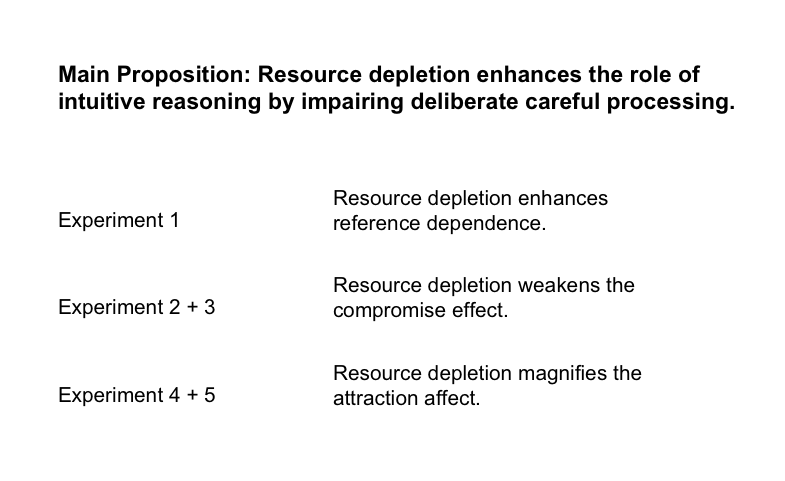
\includegraphics[width=0.9\textwidth]{images/mainpropositions.png}
  \caption{Main Propositions of the five experiments in regard to ego depletion \citep{pocheptsova2009deciding}}\label{fig:mainpropositions}
\end{figure}
Figure \ref{fig:mainpropositions} displays the result of the five experiments. Especially experiment 2 (“\emph{The ob-served effect on choice suggests that the scope of this resource is not constrained to self-regulation activities but also extends to decision-making}“ \citep[p.~350]{pocheptsova2009deciding} and experiment 3 (“\emph{[\ldots] participants whose resources are depleted by this attention regulation task will be less likely to demonstrate the compromise effect.}“ \citep[p.~350]{pocheptsova2009deciding} supports the assumption that ego depletion leads to risk-averse decision-making.\par
Unger and Stahlberg acknowledged these findings (see Figure \ref{fig:twostreams}) but also emphasised that, “\emph{[\ldots] we know little about how ego depletion affects preferences for or aversion to risky decision alternatives [\ldots]}“ \citep[p.~29]{unger2011ego}. Putting investment scenarios after a depletion task (self-regulation) at hand, Unger and Stahlberg presumed that the depleted subjects would behave risk-averse. Although the conducted experiments confirmed a decrease in risk-behaviour in general, the assumption on risk seeking and risk-avoidance strategies could not find support. 

\section{Terminology of Risk and Social Risk}
Risk as an economic concept is almost a century old (\cite{knight1921risk} in \cite{dowling1994model}). Bauer first mentioned risk in the context of consumer behaviour in 1960 (\cite{bauer1960consumer} in \cite{ross1975perceived}). However, it needed more than ten years before perceived risk was regarded as a factor of decision-making itself. „\emph{The concept of perceived risk most often used by consumer researchers defines risk in terms of the consumer's perceptions of the uncertainty and adverse consequences of buying a product (or service)}” (\cite{engel1973blackwell} in \cite{ross1975perceived}). In this way, consumer researchers implicitly assume that both the probability and the outcome of each purchase event are uncertain \citep{dowling1994model}.\par
James W. Taylor \citep{taylor1974role} understood choice as a situation in which two aspects of risk always appear side by side. He distinguished between the uncertainty regarding outcome and the uncertainty regarding consequences. Doubt on the outcome can be diminished by gathering information to make an informed decision, but when it comes to uncertainty about the consequences, risk can only be reduced when reducing the amount at stake or even cancelling the decision. Furthermore, Taylor distinguished between economic terms on the one hand and sociological or psychological terms on the other.\par
Unger and Stahlberg \citep{unger2011ego} observed two streams in the debate of ego depletion and risk. 
\begin{figure}[h!]
	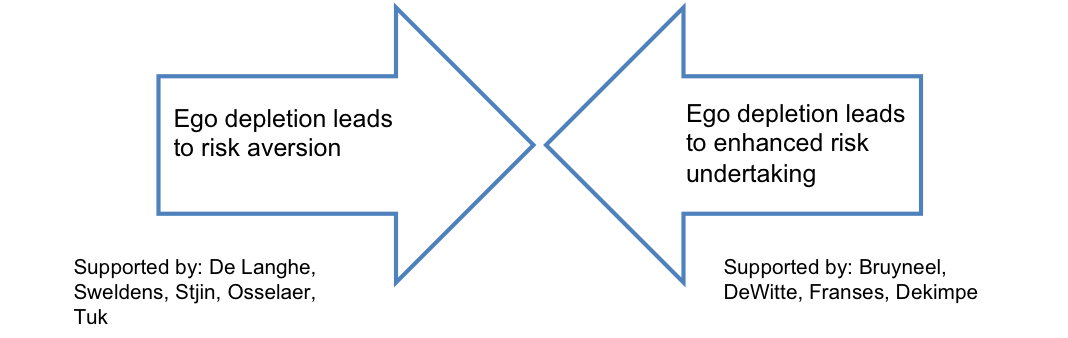
\includegraphics[width=0.9\textwidth]{images/twostreams.png}
  \caption{Two opposing trends of debate on ego depletion and social risk \citep{unger2011ego}} \label{fig:twostreams}
\end{figure}
In Unger and Stahlberg’s opinion those contradictory statements result from a different type of risk. They propose that if risk behaviour is seen in the context of gambling (uncertainty re-garding outcome), for example, ego depletion could lead to lower risk-aversion, whereas risk behaviour in decision-making processes involves the concept of responsibility (uncertainty regarding consequences), which might lead to higher risk-aversion under ego depletion. \par
Both studies aimed at a risk which can be financially interpreted and calculated, however, risk cannot always be put in clear measurable scales such as growth or currency.\par
The term ‘social risk’ can be traced back to the late 1960s where it was first identified as such in the context of decision-making. In the study of Brody and Cunningham \citep{brody1968personality} on personality-purchase behaviour relationships they simplified the consumer decision process by reckoning each variable system as a function. They established a new approach on a theoretical framework. They grouped relevant factors into four more con-trollable categories of the decision–making process.  In addition, they simplified the decision-making-process model by comprehending the relative impact of the variable system as a function of the choice condition. “\emph{Three perceptions particularly may act as filters to determine the groups of variables with the greatest weight}” \citep{brody1968personality}: (1) ‘perceived performance risk of decision-making’, (2) ‘specific self-confidence’ and (3) “\emph{[\ldots] the perceived social risk – to what extent does the person think that other people judge him by his brand decision}” \citep[p.~51]{brody1968personality}, the latter being a very plain, yet elegant definition of social risk.\par
Even though Brody and Cunningham established a definition of social risk in 1968, usage of the term varied considerably over time. Taylor \citep{taylor1974role} used uncertainty and risk as equivalent terms. Cunnings, however, observed that many writers in this field of research understood uncertainty as a concept, which is used when the likelihood is not accurately known. Even in the current debate the concept of risk appears not to have found a clear definition.\par
In this study the terminology of social risk will be narrowed down in its sense of two core aspects: (a) ‘What people think of me’ and ‘what I think of people’, when it comes to purchase decisions, and (b) the social factor of responsibility when people have to make deci-sions which possibly involve considerable consequences for others.\par
Summing up, we examined the theoretical foundation of ego depletion theory. Based on this theory, which postulates that willpower is a scarce resource that drains from the same origin as energy used in decision-making processes and self-regulation. In the debate of ego deple-tion which was strongly coined by Muraven, Tice, and Baumeister we also referred to the findings of \citep{vohs2000self,pocheptsova2009deciding,bruyneel2009felt}, who examined the consequences of ego depletion in regard to different depletion tasks, self-regulation and decision-making scenarios.\par
Special attention was paid to Unger and Stahlbergs examination in regard to the effects of ego depletion on risk behaviour \citep{unger2011ego}. Their experiment aimed to analyse risk behaviour based on financial investment scenarios. The methodical approach and the hypothesis of risk-aversive behaviour under depletion resembles to our own approach.\par
Finally, we discussed the term ‘risk’ and the meaning of it in the context of the scientific debate \citep{ross1975perceived,dowling1994model}. Furthermore we engaged in a definition of social risk, which will be the essential attribute to measure social risk in the context of decision-making.\par
The aim of this study is to observe the decision-making process in consumer behaviour under the theoretical framework of social risk. Using Baumeister’s  theory on ego depletion and Unger’s risk behaviour theory under ego depletion as the theoretical foundation, this thesis will engage in further empirical studies concerning ego depletion and the effects on consumer choice and social risk.\par
Therefore, the survey will be designed to distinguish between social risk in decision-making and social risk in decision-making concerning consumer behaviour.

